Proteins are key actors of biological processes inside cells. Rather
than carrying out tasks as single agents, they are part of dynamic
networks of protein-protein interactions (PPI) \cite{Lin2017}. Such
networks underlie a variety of interdependent mechanisms, including
signal transduction, homeostasis control and stress responses. Furthermore,
PPI networks play an important role in physiological and developmental
processes such as protein phosphorylation, transcriptional co-factor
recruitment and transporter activation \cite{Zhang2010PPI}.

A common way to create PPI networks (or validate particular protein-protein
interactions) is the \emph{Yeast-Two-Hybrid} technique (also known
as \emph{two-hybrid screening} or \emph{Y2H}). Figure \ref{Y2H}A
illustrates the biological basis of Y2H: the expression of a specific
reporter gene is activated by the binding of a DNA-binding Domain
(DB) and an Activation Domain (AD) of a Transcription Factor, which
in turn binds to an Upstream Activation Sequence (UAS). To evaluate
an interaction between two proteins, the Y2H approach fuses one protein
to the DB domain (known as \emph{bait}) and another protein to the
AD (known as \emph{prey}). If the proteins interact, the reporter
gene expression is activated by the AD (Fig. \ref{Y2H}B). Otherwise,
if proteins fail to interact, the reporter gene is not expressed (Fig.
\ref{Y2H}C).

\begin{figure}[h]
\caption{\label{Y2H}The Yeast-2-Hybrid technique offers an experimental approach
for constructing PPI networks.}

%\noindent \centering{}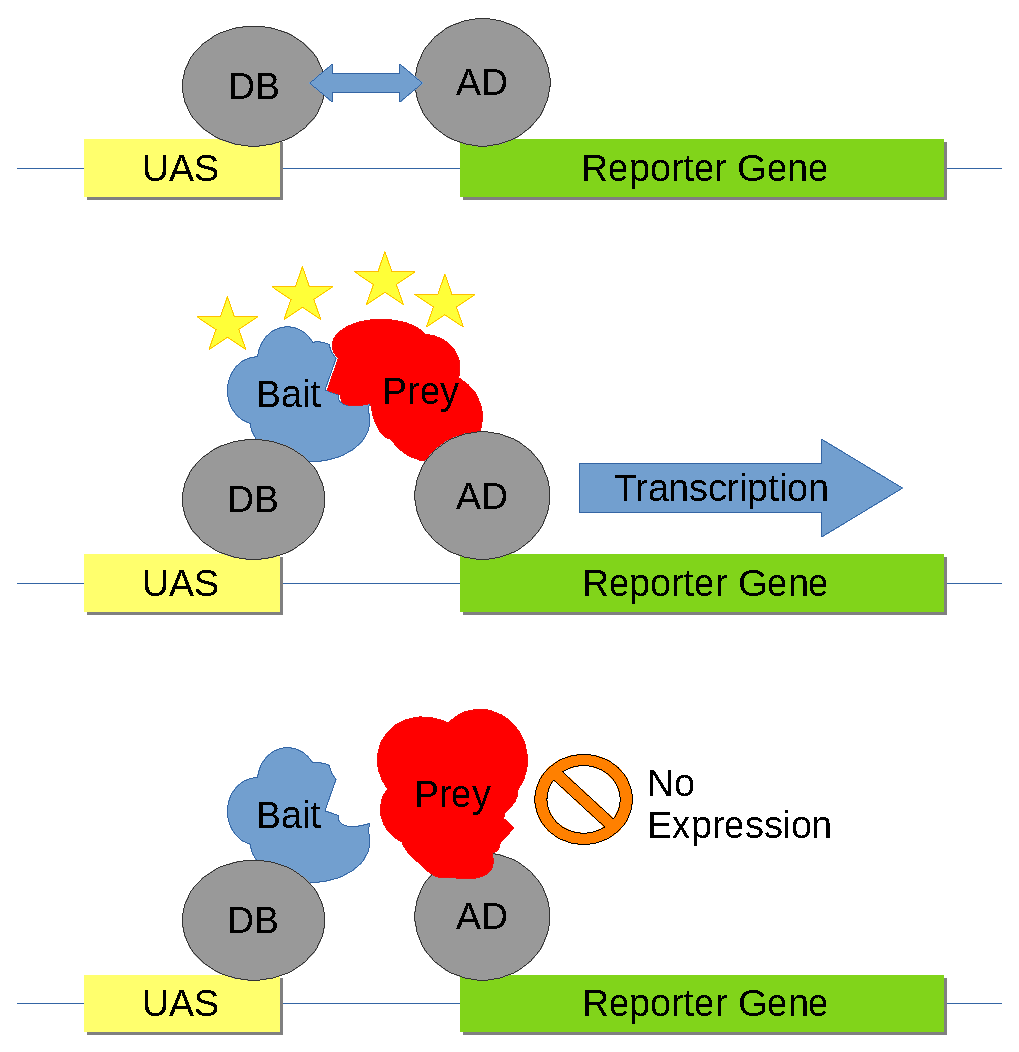
\includegraphics[width=0.7\columnwidth]{Y2H}
\end{figure}

Based on the outcome of numerous Y2H experiments, undirected networks
of interactions between proteins can be constructed. However, relying
only on experimental validation of PPIs is detrimental to research
due to its hindrance in costs, accuracy, required manpower and time
\cite{Laraia2015PPI,Macalino2018PPI}. Besides, the number of missing
interactions for pairs of proteins on many organisms leverage the
usage of computational methods for prediction of such interactions.

A common way of predicting interactions is usually based on social
networks analysis, more specifically on the triadic closure principle
(TCP). TCP states that the higher the number of common neighboring
nodes between two nodes, the higher the probability that they interact
\cite{Goldberg2003SmallWorld}. TCP can be addressed mathematically
by counting the number of shared neighbors of a pair of nodes, also
known as the Common Neighbors algorithm. By raising the adjacency
matrix (A) of the network to the second power (A\texttwosuperior ),
TCP can be considered for further analyses. However, previous studies
show that the mentioned approach usually fails because it does not
consider the structural and chemical properties of the proteins \cite{Cannistraci2013Networks,Kovacs2019}.

A variety of methods for predicting interactions in PPI networks have
been proposed in recent years \cite{Chang2016PPI,Chen2019PPI,Kotlyar2015PPI}.
Kovacs et al (2019) introduce a network-based approach which predicts
the interaction between two proteins based on the number of paths
of length 3, normalized by the geometric average of their interactions.
The simplest mathematical representation of this principle consists
on the third power of the adjacency matrix (A\textthreesuperior).
Furthermore, Kovacs et al present a degree-normalized scaling for
this metric, which reduces bias caused by intermediate hubs within
the paths of length 3. This handcrafted measure, denoted L3, enables
the proposed approach to outperform previous methods for predicting
binary protein interactions in yeast (\emph{S. cerevisiae}), Arabidopsis
(\emph{A. thaliana}), worm (\emph{C. elegans}), fly (\emph{D. melanogaster}),
fission yeast (\emph{S. pombe}), mouse (\emph{M. musculus}) and humans
\cite{Kovacs2019}.


The focus of this study is to evaluate different methods for predicting
PPIs using the network of known interactions. To achieve this, human
and rice PPI networks are compared using the proposed methods (A2,
A3, L3), as well as a low-dimensional representation of nodes (\texttt{Node2Vec})\cite{Grover_2016}.
After that, combinations of the two types of methods are tested. In
the case of the human network, two different versions of the human
interactome \cite{Rolland2014Human} are used for training and another
interactome version is used for validation (\emph{HI-III})\cite{Kovacs2019}.
For the rice interactome, a portion of the known interactions removed
and then predicted with different techniques based on the known interactions.
The main contributions of this paper are i) a general framework for
link prediction in non-directed networks and ii) two applications
of this framework to biological networks with a structural insight.

\paragraph*{Structure:} This paper is organized as follows. \emph{Materials and Methods} describes
the methodological steps and key milestones in the preparation of
the networks, model parameters and experimental configurations.
\emph{Results} presents the main results of the models for the human and rice interactomes.
\emph{Conclussions} presents the main conclusions of this study. Finally, \emph{Appendix}
presents supplementary information and figures which complement the
results described in this paper.